\chapter{PK5 --- Mâm cơm}
\begin{figure}[H]\centering
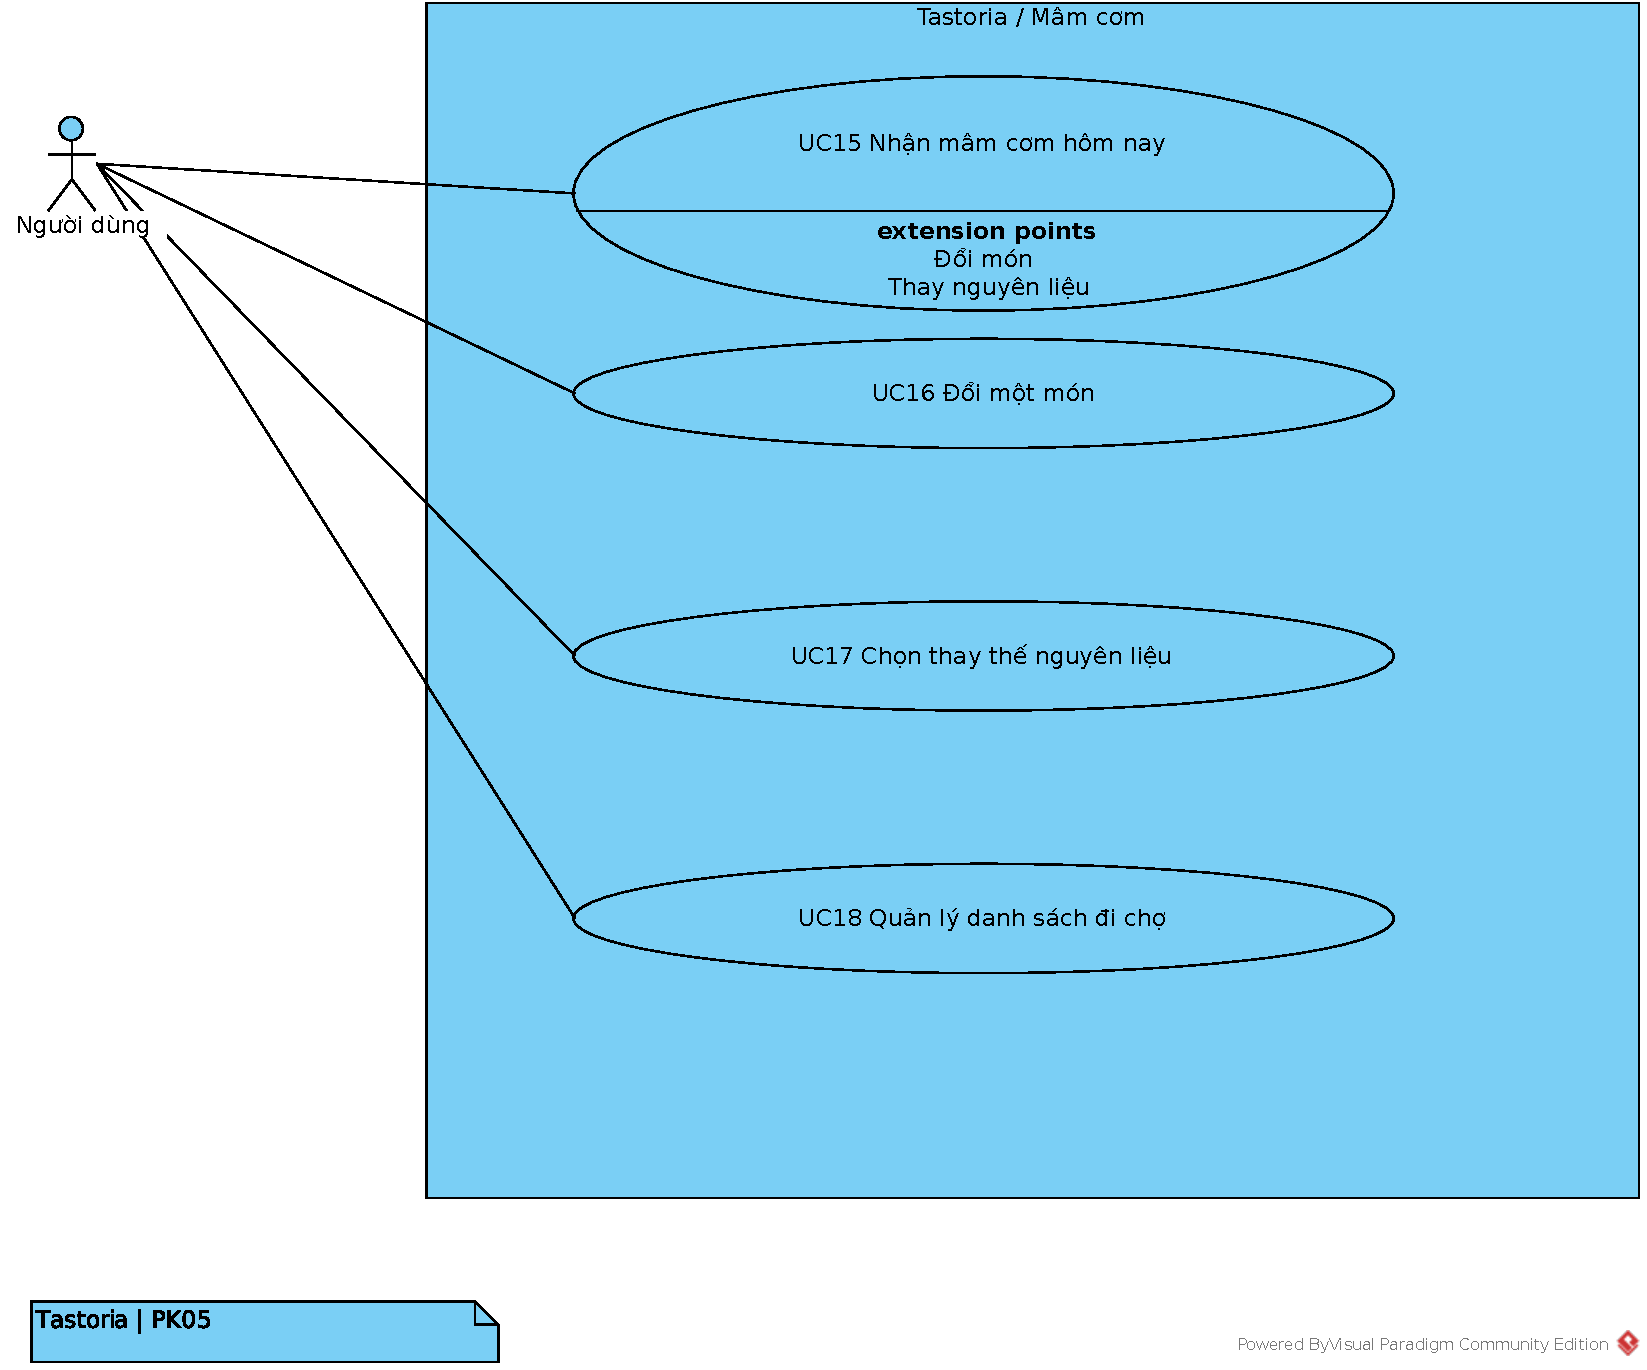
\includegraphics[width=0.96\linewidth,height=0.75\textheight,keepaspectratio]{assets/PK05.pdf}
\caption{PK05 --- Phân rã use case}\label{fig:Phu-luc-A-Use-Cases:5}
\end{figure}
\section{UC15 --- Nhận mâm cơm hôm nay}
\subsection{Mục tiêu trong ngữ cảnh}
Người dùng (A02) muốn biết bữa trưa hoặc bữa tối nay nấu gì. Hệ thống ghép một mâm cơm Việt (mặn + rau + canh, hoặc 2 món khi ăn một mình) từ nguyên liệu đang có trong kho, ưu tiên lô sắp hỏng, hợp gu, vừa năng lượng mục tiêu, nấu xong trong thời gian người dùng chọn, và không chứa thứ gì thuộc nhóm dị ứng hoặc trái chế độ ăn của người dùng và người ăn cùng.

\subsection{Phạm vi và mức}
\begin{itemize}
\item Phạm vi: hệ thống Tastoria (app Android/\allowbreak{}web + backend), hộp đen.
\item Mức: mục tiêu người dùng (user goal, mức "mặt biển").
\item Gói: PK5 Mâm cơm.
\end{itemize}
\subsection{Tác nhân và bên liên quan (quyền lợi)}
{\footnotesize\setlength{\tabcolsep}{0pt}
\begin{longtable}{@{}L{7.850cm}@{\hspace{3mm}}L{7.850cm}@{}}
\caption{Tác nhân và bên liên quan (quyền lợi)}\\
\toprule
\textbf{Bên liên quan} & \textbf{Quyền lợi} \\
\midrule\endfirsthead
\multicolumn{2}{l}{\small\itshape Bảng \thetable{} (tiếp theo)}\\
\toprule
\textbf{Bên liên quan} & \textbf{Quyền lợi} \\
\midrule\endhead
\bottomrule\endfoot
A02 Người dùng (tác nhân chính) & Có mâm nấu được ngay bằng đồ đang có, ít phải đi chợ, dùng kịp đồ sắp hỏng, bám mục tiêu calo. \\ \addlinespace[3pt]
Người ăn cùng (không có tài khoản, khai qua A02) & Không bị đề xuất món, gia vị hay đồ thay thế thuộc nhóm dị ứng của mình. \\ \addlinespace[3pt]
Nhóm dự án (học máy) & Có tương tác {\small\texttt{served}}/\allowbreak{}{\small\texttt{viewed}} hợp lệ, gắn phiên bản bộ xếp hạng và xác suất hiển thị, để huấn luyện lại; chỉ khi người dùng đồng ý {\small\texttt{personalization}}. \\ \addlinespace[3pt]
Bên kiểm soát dữ liệu & Dữ liệu sức khoẻ chỉ được giải mã trong module profile và có nhật ký kiểm toán; không ghi dữ liệu hành vi khi thiếu đồng ý. \\ \addlinespace[3pt]
\end{longtable}}
\subsection{Tiền điều kiện}
\begin{enumerate}
\item A02 đã đăng nhập (UC02), có access token còn hạn.
\item Kho món có ít nhất một món {\small\texttt{published}} cho mỗi slot {\small\texttt{man}}, {\small\texttt{rau}}, {\small\texttt{canh}}.
\end{enumerate}
Việc A02 đã hoàn tất UC09 hay chưa không phải tiền điều kiện: hệ thống không bảo đảm điều đó trước khi UC bắt đầu, nên trường hợp chưa có hồ sơ được xử lý ở mở rộng 1a.

\subsection{Đảm bảo tối thiểu}
\begin{itemize}
\item Không có mâm nào được lưu hoặc trả về nếu vi phạm BR-\allowbreak{}ALG-\allowbreak{}01 hoặc BR-\allowbreak{}DIET-\allowbreak{}01.
\item Không có bản ghi {\small\texttt{interactions}} nào được ghi khi A02 chưa đồng ý (hoặc đã rút đồng ý) mục đích {\small\texttt{personalization}}.
\item Kho ({\small\texttt{pantry\_\allowbreak{}\allowbreak{}lots}}, {\small\texttt{pantry\_\allowbreak{}\allowbreak{}transactions}}) không thay đổi: UC15 chỉ đọc kho.
\item Gửi lại cùng {\small\texttt{Idempotency-\allowbreak{}Key}} không tạo mâm thứ hai.
\end{itemize}
\subsection{Đảm bảo khi thành công}
\begin{itemize}
\item Có một bản ghi {\small\texttt{meal\_\allowbreak{}\allowbreak{}plans}} trạng thái {\small\texttt{proposed}} (sau bước chấp nhận là {\small\texttt{accepted}}) của A02, kèm 2 hoặc 3 dòng {\small\texttt{meal\_\allowbreak{}\allowbreak{}plan\_\allowbreak{}\allowbreak{}items}} trạng thái {\small\texttt{active}} (mỗi slot tối đa một dòng), dị ứng người ăn cùng ({\small\texttt{meal\_\allowbreak{}\allowbreak{}plan\_\allowbreak{}\allowbreak{}coeater\_\allowbreak{}\allowbreak{}allergens}}), lô ghim ({\small\texttt{meal\_\allowbreak{}\allowbreak{}plan\_\allowbreak{}\allowbreak{}pins}}), ảnh chụp mục tiêu năng lượng, số bát cơm gợi ý, dòng lý do, phiên bản bộ xếp hạng và phiên bản tham số.
\item Mâm thoả BR-\allowbreak{}TRAY-\allowbreak{}01, BR-\allowbreak{}TRAY-\allowbreak{}04, BR-\allowbreak{}TRAY-\allowbreak{}05, BR-\allowbreak{}TRAY-\allowbreak{}08, BR-\allowbreak{}ALG-\allowbreak{}01, BR-\allowbreak{}DIET-\allowbreak{}01.
\item Nếu A02 đã đồng ý {\small\texttt{personalization}}: có một {\small\texttt{interactions}} loại {\small\texttt{served}} cho mỗi món trong mâm.
\end{itemize}
\subsection{Kích hoạt}
A02 bấm "Ra mâm cơm" ở màn Xác nhận nguyên liệu (sau UC13) hoặc nút "Mâm cơm hôm nay" ở Trang chủ.

\subsection{Kịch bản chính}
Kịch bản viết ở mức tác nhân \ensuremath{\leftrightarrow} hệ thống (hộp đen). Lời gọi giữa các module, bảng và view được đọc ở từng bước nằm ở sơ đồ tuần tự {\small\texttt{docs/\allowbreak{}\allowbreak{}uml/\allowbreak{}\allowbreak{}sequence/\allowbreak{}\allowbreak{}SD03-\allowbreak{}tao-\allowbreak{}mam.\allowbreak{}puml}} và mục 13 (Dữ liệu); chúng là thiết kế, không phải yêu cầu.

\begin{enumerate}
\item A02 mở màn Mâm cơm hôm nay. App hiện danh mục nhóm dị ứng, các lô đang có trong kho và điền sẵn số người mặc định của A02.
\item A02 chọn bữa (trưa/\allowbreak{}tối), số người n, thời gian nấu tối đa, (tuỳ chọn) nhóm dị ứng của người ăn cùng và tối đa 2 lô "phải dùng", rồi bấm "Ra mâm".
\item App gửi yêu cầu tạo mâm kèm một khoá lũy đẳng mới ({\small\texttt{POST /\allowbreak{}\allowbreak{}meal-\allowbreak{}plans}}, header {\small\texttt{Idempotency-\allowbreak{}Key}}).
\item Hệ thống kiểm khoá lũy đẳng và dữ liệu vào (FR-\allowbreak{}15-\allowbreak{}01 \ldots{} FR-\allowbreak{}15-\allowbreak{}05).
\item Hệ thống lấy ràng buộc bữa ăn của A02: nhóm dị ứng, chế độ ăn, số họng bếp, 5 món hay ăn và E\_\allowbreak{}mâm của bữa đã chọn (BR-\allowbreak{}NUT-\allowbreak{}04). Mỗi lần đọc chỉ số sức khoẻ để tính E\_\allowbreak{}mâm được ghi nhật ký kiểm toán.
\item Hệ thống kiểm A02 có đồng ý {\small\texttt{personalization}} hiện hành hay không.
\item Hệ thống xác định lượng khả dụng của từng lô trong kho A02 và độ gấp u tại thời điểm này; lô ở mức "kiểm tra trước khi dùng" không được tính (BR-\allowbreak{}FRESH-\allowbreak{}04).
\item Hệ thống lọc cứng các món {\small\texttt{published}}, loại món có nguyên liệu thuộc nhóm dị ứng của A02 hoặc người ăn cùng, hoặc trái chế độ ăn của A02 (BR-\allowbreak{}ALG-\allowbreak{}01, BR-\allowbreak{}DIET-\allowbreak{}01).
\item Hệ thống chấm điểm gu cho từng món còn lại (FR-\allowbreak{}15-\allowbreak{}17, FR-\allowbreak{}15-\allowbreak{}18).
\item Hệ thống ghép mâm: trong các tổ hợp thoả BR-\allowbreak{}TRAY-\allowbreak{}01, BR-\allowbreak{}TRAY-\allowbreak{}04, BR-\allowbreak{}TRAY-\allowbreak{}05 và BR-\allowbreak{}TRAY-\allowbreak{}08, chọn tổ hợp có hàm mục tiêu cao nhất (FR-\allowbreak{}15-\allowbreak{}14, FR-\allowbreak{}15-\allowbreak{}15).
\item Hệ thống tính số bát cơm gợi ý (BR-\allowbreak{}TRAY-\allowbreak{}03), khoảng calo (BR-\allowbreak{}NUT-\allowbreak{}06) và dòng lý do.
\item Hệ thống lưu mâm ở trạng thái {\small\texttt{proposed}}, ghi tương tác {\small\texttt{served}} nếu A02 có đồng ý {\small\texttt{personalization}}, ghi nhớ phản hồi theo khoá lũy đẳng và trả mâm (201).
\item App hiện mâm tròn: tên món, dòng lý do, thanh calo dạng khoảng so với mục tiêu (ghi "xấp xỉ theo số người"), "gợi ý x bát cơm".
\item A02 chạm một món để xem chi tiết; app lấy chi tiết món ({\small\texttt{GET /\allowbreak{}\allowbreak{}recipes/\allowbreak{}\allowbreak{}\{id\}}}) và gửi sự kiện {\small\texttt{viewed}} ({\small\texttt{POST /\allowbreak{}\allowbreak{}events}}).
\item A02 bấm "Nấu mâm này"; app gửi {\small\texttt{POST /\allowbreak{}\allowbreak{}meal-\allowbreak{}plans/\allowbreak{}\allowbreak{}\{id\}/\allowbreak{}\allowbreak{}accept}}; hệ thống chuyển mâm sang {\small\texttt{accepted}}. App chuyển sang UC19.
\end{enumerate}
\subsection{Mở rộng}
\begin{itemize}
\item \textbf{1a. A02 chưa hoàn tất UC09} (chưa có hồ sơ hoặc cài đặt bếp): app hiện nhắc "Bạn chưa khai dị ứng và mục tiêu" kèm nút mở UC09 trước khi cho bấm "Ra mâm". Nếu A02 vẫn ra mâm, hệ thống ghép mâm như với người chưa khai dị ứng, chưa chọn chế độ ăn, không có mục tiêu năng lượng (như 5a) và dùng giá trị mặc định của cài đặt bếp (FR-\allowbreak{}15-\allowbreak{}36). Tiếp bước 2.
\item \textbf{1b. Mở lại app khi đã có mâm}: app gọi {\small\texttt{GET /\allowbreak{}\allowbreak{}meal-\allowbreak{}plans/\allowbreak{}\allowbreak{}latest}}; nếu có mâm thì hiện mâm đó và tiếp từ bước 13; nếu 404 thì tiếp bước 2.
\item \textbf{2a. A02 muốn tự chọn món}: app cho xem danh sách món qua {\small\texttt{GET /\allowbreak{}\allowbreak{}recipes}} để tham khảo; việc thay món trong mâm thực hiện ở UC16 sau bước 13.
\item \textbf{4a. Dữ liệu vào sai} (n ngoài [1, 6], thời gian ngoài [10, 180] phút, bữa không hợp lệ, quá 2 lô ghim, lô ghim không thuộc A02 hoặc không {\small\texttt{in\_\allowbreak{}\allowbreak{}stock}}, mã dị ứng người ăn cùng không có trong {\small\texttt{allergen\_\allowbreak{}\allowbreak{}groups}}): API trả 422 với {\small\texttt{code}} riêng từng lỗi; không lưu gì; app tô đỏ trường lỗi, A02 sửa và quay lại bước 3.
\item \textbf{4b. Thiếu header {\small\texttt{Idempotency-\allowbreak{}Key}}}: API trả 400; app (lỗi lập trình) ghi log và sinh khoá rồi gửi lại.
\item \textbf{4c. Gửi lại cùng khoá, cùng nội dung} (mất mạng sau bước 3, app gửi lại khi có mạng; hoặc bấm hai lần): hệ thống trả nguyên văn phản hồi đã lưu (mã trạng thái và thân); không tạo mâm mới. Tiếp bước 13.
\item \textbf{4d. Cùng khoá, khác nội dung}: API trả 422 {\small\texttt{idempotency\_\allowbreak{}\allowbreak{}key\_\allowbreak{}\allowbreak{}reused}}; app sinh khoá mới cho yêu cầu mới.
\item \textbf{4e. Yêu cầu đầu tiên còn đang xử lý khi bản gửi lại tới}: API trả 409 kèm {\small\texttt{Retry-\allowbreak{}After}}; app chờ rồi gửi lại cùng khoá.
\item \textbf{5a. Chưa đồng ý {\small\texttt{health\_\allowbreak{}\allowbreak{}profile}} hoặc chưa có mục tiêu năng lượng}: hệ thống không có E\_\allowbreak{}mâm; đặt \ensuremath{\beta} = 0, {\small\texttt{e\_\allowbreak{}\allowbreak{}target\_\allowbreak{}\allowbreak{}kcal}}, {\small\texttt{rice\_\allowbreak{}\allowbreak{}bowls\_\allowbreak{}\allowbreak{}per\_\allowbreak{}\allowbreak{}person}} = NULL; app hiện "chưa có mục tiêu" và nút mở UC11 (BR-\allowbreak{}CONSENT-\allowbreak{}02). Tiếp bước 6.
\item \textbf{6a. Chưa đồng ý {\small\texttt{personalization}}}: hệ thống xếp hạng bằng trung bình món + content-\allowbreak{}based từ 5 món hay ăn, không đọc {\small\texttt{interactions}}; ở bước 12 không ghi {\small\texttt{served}} (BR-\allowbreak{}CONSENT-\allowbreak{}03).
\item \textbf{9a. Không có bản bộ xếp hạng đang triển khai hoặc nạp lỗi}: hệ thống dùng trung bình món + content-\allowbreak{}based như 6a, ghi {\small\texttt{ranker\_\allowbreak{}\allowbreak{}version\_\allowbreak{}\allowbreak{}id}} = NULL; tiếp bước 10.
\item \textbf{10a. Không có mâm 3 món khả thi khi n \ensuremath{\geq} 2}: hệ thống thử mâm 2 món (mặn + rau hoặc canh). Có thì tiếp bước 11, dòng lý do ghi rõ "mâm 2 món vì thiếu nguyên liệu" (BR-\allowbreak{}TRAY-\allowbreak{}06, FR-\allowbreak{}15-\allowbreak{}24).
\item \textbf{10b. Vẫn không có mâm khả thi}: API trả 422 {\small\texttt{no\_\allowbreak{}\allowbreak{}feasible\_\allowbreak{}\allowbreak{}tray}} kèm danh sách nguyên liệu còn thiếu (gam) của 3 mâm có hàm mục tiêu cao nhất bỏ qua ràng buộc kho; không lưu {\small\texttt{meal\_\allowbreak{}\allowbreak{}plans}} (FR-\allowbreak{}15-\allowbreak{}31). App hiện danh sách; điểm mở rộng tới \textbf{UC18} (điều kiện "không có mâm khả thi (BR-\allowbreak{}TRAY-\allowbreak{}06)"): A02 chọn nguyên liệu để đưa vào danh sách đi chợ.
\item \textbf{10c. Lô ghim không thể dùng đủ 50\% g\_\allowbreak{}min trong mâm khả thi nào}: API trả 422 {\small\texttt{pin\_\allowbreak{}\allowbreak{}unsatisfiable}} nêu lô gây xung đột; app gợi ý bỏ ghim lô đó; A02 bỏ ghim và quay lại bước 3 với khoá mới (BR-\allowbreak{}TRAY-\allowbreak{}08, FR-\allowbreak{}15-\allowbreak{}30).
\item \textbf{10d. Không có mâm nào nấu xong trong thời gian tối đa}: xử lý như 10a/\allowbreak{}10b; danh sách thiếu ghi lý do "thời gian"; app gợi ý tăng thời gian tối đa.
\item \textbf{12a. Quá thời gian chờ phía app} (không nhận phản hồi sau 10 s): app hiện "đang ghép mâm", gửi lại cùng {\small\texttt{Idempotency-\allowbreak{}Key}} (như 4c/\allowbreak{}4e), tối đa 3 lần rồi báo lỗi mạng và giữ dữ liệu đã nhập.
\item \textbf{12b. Lỗi hệ thống} (DB, lỗi không lường): giao dịch rollback, không lưu mâm, không lưu khoá lũy đẳng; API trả 500 RFC 9457 có {\small\texttt{request\_\allowbreak{}\allowbreak{}id}}; app hiện "chưa ghép được mâm, thử lại" và cho gửi lại cùng khoá.
\item \textbf{13a. A02 không ưng một món}: điểm mở rộng tới \textbf{UC16} (Đổi một món).
\item \textbf{13b. A02 muốn xem thiếu gì /\allowbreak{} thay nguyên liệu của một món}: điểm mở rộng tới \textbf{UC17}.
\item \textbf{14a. Mất mạng khi gửi {\small\texttt{viewed}}}: app giữ sự kiện trong outbox với {\small\texttt{event\_\allowbreak{}\allowbreak{}id}} cố định, gửi lại khi có mạng; hệ thống bỏ qua bản trùng theo {\small\texttt{event\_\allowbreak{}\allowbreak{}id}}.
\item \textbf{15a. Mâm không còn ở {\small\texttt{proposed}}} (đã {\small\texttt{cooked}}, {\small\texttt{abandoned}}, {\small\texttt{expired}}): API trả 409 (FR-\allowbreak{}15-\allowbreak{}33); app tải lại mâm bằng {\small\texttt{GET /\allowbreak{}\allowbreak{}meal-\allowbreak{}plans/\allowbreak{}\allowbreak{}\{id\}}}.
\item \textbf{15b. Gửi lại accept khi mâm đã {\small\texttt{accepted}}}: API trả 200 với mâm hiện tại, không đổi gì (FR-\allowbreak{}15-\allowbreak{}32).
\item \textbf{15c. A02 không nấu mâm này}: khi A02 tạo mâm mới cho cùng bữa, hoặc khi đã qua giờ kết thúc bữa, mâm {\small\texttt{proposed}} chuyển {\small\texttt{expired}} và mâm {\small\texttt{accepted}} chưa có phiên nấu {\small\texttt{in\_\allowbreak{}\allowbreak{}progress}} chuyển {\small\texttt{abandoned}} (FR-\allowbreak{}15-\allowbreak{}37 \ldots{} FR-\allowbreak{}15-\allowbreak{}39, FR-\allowbreak{}15-\allowbreak{}41; sơ đồ ST02).
\item \textbf{*a. Truy cập mâm của người khác} ({\small\texttt{GET /\allowbreak{}\allowbreak{}meal-\allowbreak{}plans/\allowbreak{}\allowbreak{}\{id\}}}, accept): API trả 404 (chống BOLA; FR-\allowbreak{}15-\allowbreak{}28, FR-\allowbreak{}15-\allowbreak{}34).
\item \textbf{*b. Access token hết hạn}: app làm mới phiên (UC02, {\small\texttt{POST /\allowbreak{}\allowbreak{}auth/\allowbreak{}\allowbreak{}refresh}}) rồi gửi lại yêu cầu với cùng {\small\texttt{Idempotency-\allowbreak{}Key}}.
\end{itemize}
\subsection{Ghi chú đối chiếu của báo cáo}
Hai điểm mở rộng Đổi món và Thay nguyên liệu của UC15 dành cho UC16 và UC17. Các ràng buộc dị ứng/\allowbreak{}kho/\allowbreak{}thời gian phải được kiểm toàn mâm, không chỉ từng món.

\textbf{Nguồn:} {\small\texttt{Tastoria/\allowbreak{}\allowbreak{}docs/\allowbreak{}\allowbreak{}sad/\allowbreak{}\allowbreak{}use-\allowbreak{}cases/\allowbreak{}\allowbreak{}UC15.\allowbreak{}md}}. Mã nghiệp vụ: BR-\allowbreak{}TRAY-\allowbreak{}01, BR-\allowbreak{}TRAY-\allowbreak{}02, BR-\allowbreak{}TRAY-\allowbreak{}03, BR-\allowbreak{}TRAY-\allowbreak{}04, BR-\allowbreak{}TRAY-\allowbreak{}05, BR-\allowbreak{}TRAY-\allowbreak{}06, BR-\allowbreak{}TRAY-\allowbreak{}07, BR-\allowbreak{}TRAY-\allowbreak{}08, BR-\allowbreak{}ALG-\allowbreak{}01, BR-\allowbreak{}DIET-\allowbreak{}01, BR-\allowbreak{}NUT-\allowbreak{}04, BR-\allowbreak{}NUT-\allowbreak{}06, BR-\allowbreak{}CONSENT-\allowbreak{}03, BR-\allowbreak{}CONSENT-\allowbreak{}02, BR-\allowbreak{}FRESH-\allowbreak{}04, BR-\allowbreak{}FRESH-\allowbreak{}05, BR-\allowbreak{}QTY-\allowbreak{}01, BR-\allowbreak{}QTY-\allowbreak{}02, BR-\allowbreak{}COOK-\allowbreak{}01, BR-\allowbreak{}CATALOG-\allowbreak{}01.

\textbf{Dữ liệu liên quan:} {\small\texttt{meal\_\allowbreak{}\allowbreak{}plans}}, {\small\texttt{meal\_\allowbreak{}\allowbreak{}plan\_\allowbreak{}\allowbreak{}items}}, {\small\texttt{meal\_\allowbreak{}\allowbreak{}plan\_\allowbreak{}\allowbreak{}coeater\_\allowbreak{}\allowbreak{}allergens}}, {\small\texttt{meal\_\allowbreak{}\allowbreak{}plan\_\allowbreak{}\allowbreak{}pins}}, {\small\texttt{meal\_\allowbreak{}\allowbreak{}plan\_\allowbreak{}\allowbreak{}item\_\allowbreak{}\allowbreak{}substitutions}}, {\small\texttt{idempotency\_\allowbreak{}\allowbreak{}keys}}, {\small\texttt{profiles}}, {\small\texttt{user\_\allowbreak{}\allowbreak{}allergens}}, {\small\texttt{user\_\allowbreak{}\allowbreak{}favorite\_\allowbreak{}\allowbreak{}recipes}}, {\small\texttt{user\_\allowbreak{}\allowbreak{}settings}}, {\small\texttt{allergen\_\allowbreak{}\allowbreak{}groups}}, {\small\texttt{diets}}, {\small\texttt{diet\_\allowbreak{}\allowbreak{}exclusions}}, {\small\texttt{food\_\allowbreak{}\allowbreak{}groups}}, {\small\texttt{ingredients}}, {\small\texttt{ingredient\_\allowbreak{}\allowbreak{}allergens}}, {\small\texttt{ingredient\_\allowbreak{}\allowbreak{}units}}, {\small\texttt{recipes}}, {\small\texttt{recipe\_\allowbreak{}\allowbreak{}ingredients}}, {\small\texttt{recipe\_\allowbreak{}\allowbreak{}steps}}, {\small\texttt{recipe\_\allowbreak{}\allowbreak{}nutrition}}, {\small\texttt{recipe\_\allowbreak{}\allowbreak{}tags}}, {\small\texttt{recipe\_\allowbreak{}\allowbreak{}sources}}, {\small\texttt{tags}}, {\small\texttt{cooking\_\allowbreak{}\allowbreak{}methods}}, {\small\texttt{food\_\allowbreak{}\allowbreak{}items}}, {\small\texttt{food\_\allowbreak{}\allowbreak{}nutrients}}, {\small\texttt{nutrients}}, {\small\texttt{pantry\_\allowbreak{}\allowbreak{}lots}}, {\small\texttt{v\_\allowbreak{}\allowbreak{}pantry\_\allowbreak{}\allowbreak{}lot\_\allowbreak{}\allowbreak{}balance}}, {\small\texttt{substitution\_\allowbreak{}\allowbreak{}pairs}}, {\small\texttt{model\_\allowbreak{}\allowbreak{}deployments}}, {\small\texttt{model\_\allowbreak{}\allowbreak{}versions}}, {\small\texttt{interactions}}, {\small\texttt{v\_\allowbreak{}\allowbreak{}current\_\allowbreak{}\allowbreak{}consents}}, {\small\texttt{audit\_\allowbreak{}\allowbreak{}log}}.

\textbf{Điểm giao tiếp:} {\small\texttt{POST /\allowbreak{}\allowbreak{}meal-\allowbreak{}plans}}; {\small\texttt{GET /\allowbreak{}\allowbreak{}meal-\allowbreak{}plans/\allowbreak{}\allowbreak{}latest}}; {\small\texttt{GET /\allowbreak{}\allowbreak{}meal-\allowbreak{}plans/\allowbreak{}\allowbreak{}\{id\}}}; {\small\texttt{POST /\allowbreak{}\allowbreak{}meal-\allowbreak{}plans/\allowbreak{}\allowbreak{}\{id\}/\allowbreak{}\allowbreak{}accept}}; {\small\texttt{GET /\allowbreak{}\allowbreak{}pantry/\allowbreak{}\allowbreak{}lots}}; {\small\texttt{GET /\allowbreak{}\allowbreak{}reference}}; {\small\texttt{GET /\allowbreak{}\allowbreak{}recipes}}; {\small\texttt{GET /\allowbreak{}\allowbreak{}recipes/\allowbreak{}\allowbreak{}\{id\}}}; {\small\texttt{POST /\allowbreak{}\allowbreak{}events}}.

\section{UC16 --- Đổi một món}
\subsection{Mục tiêu trong ngữ cảnh}
Trong mâm vừa nhận (UC15), A02 không muốn một món. A02 chọn lý do; hệ thống thay đúng món đó bằng món khác cùng slot, giữ nguyên các món còn lại, và mâm mới vẫn khả thi về kho, thời gian, lô ghim, dị ứng và chế độ ăn. Lý do đổi được lưu để phân biệt nhãn âm về gu ("không hợp gu") với các lý do ngữ cảnh.

\subsection{Phạm vi và mức}
\begin{itemize}
\item Phạm vi: hệ thống Tastoria, hộp đen.
\item Mức: mục tiêu con (subfunction) mở rộng UC15 ({\small\texttt{extend: UC15}}).
\item Gói: PK5 Mâm cơm.
\end{itemize}
\subsection{Tác nhân và bên liên quan (quyền lợi)}
{\footnotesize\setlength{\tabcolsep}{0pt}
\begin{longtable}{@{}L{7.850cm}@{\hspace{3mm}}L{7.850cm}@{}}
\caption{Tác nhân và bên liên quan (quyền lợi)}\\
\toprule
\textbf{Bên liên quan} & \textbf{Quyền lợi} \\
\midrule\endfirsthead
\multicolumn{2}{l}{\small\itshape Bảng \thetable{} (tiếp theo)}\\
\toprule
\textbf{Bên liên quan} & \textbf{Quyền lợi} \\
\midrule\endhead
\bottomrule\endfoot
A02 Người dùng (tác nhân chính) & Đổi nhanh một món mà không mất các món đã ưng; không gặp lại món vừa bỏ trong cùng mâm. \\ \addlinespace[3pt]
Người ăn cùng (khai qua A02) & Món mới vẫn tránh nhóm dị ứng đã khai cho bữa này. \\ \addlinespace[3pt]
Nhóm dự án (học máy) & Lý do đổi được ghi đúng; chỉ "không hợp gu" là nhãn âm về gu; chỉ ghi khi có đồng ý {\small\texttt{personalization}}. \\ \addlinespace[3pt]
\end{longtable}}
\subsection{Tiền điều kiện}
\begin{enumerate}
\item A02 đã đăng nhập.
\item Có mâm của A02 ở trạng thái {\small\texttt{proposed}} hoặc {\small\texttt{accepted}}, và món cần đổi là {\small\texttt{meal\_\allowbreak{}\allowbreak{}plan\_\allowbreak{}\allowbreak{}items}} {\small\texttt{active}} của mâm đó.
\end{enumerate}
\subsection{Đảm bảo tối thiểu}
\begin{itemize}
\item Mâm luôn có đúng một món {\small\texttt{active}} cho mỗi slot đang có (ràng buộc {\small\texttt{UNIQUE(meal\_\allowbreak{}\allowbreak{}plan\_\allowbreak{}\allowbreak{}id, slot) WHERE status = 'active'}}).
\item Không món mới nào vi phạm BR-\allowbreak{}ALG-\allowbreak{}01, BR-\allowbreak{}DIET-\allowbreak{}01.
\item Nếu không đổi được, mâm giữ nguyên như trước yêu cầu.
\item Gửi lại cùng {\small\texttt{Idempotency-\allowbreak{}Key}} không đổi món lần thứ hai.
\end{itemize}
\subsection{Đảm bảo khi thành công}
\begin{itemize}
\item Dòng món cũ chuyển {\small\texttt{swapped\_\allowbreak{}\allowbreak{}out}}, ghi {\small\texttt{swap\_\allowbreak{}\allowbreak{}reason}}; có dòng món mới {\small\texttt{active}} cùng slot, {\small\texttt{replaced\_\allowbreak{}\allowbreak{}item\_\allowbreak{}\allowbreak{}id}} trỏ dòng cũ.
\item {\small\texttt{meal\_\allowbreak{}\allowbreak{}plans.\allowbreak{}kcal\_\allowbreak{}\allowbreak{}low}}, {\small\texttt{kcal\_\allowbreak{}\allowbreak{}high}}, {\small\texttt{rice\_\allowbreak{}\allowbreak{}bowls\_\allowbreak{}\allowbreak{}per\_\allowbreak{}\allowbreak{}person}}, {\small\texttt{reason\_\allowbreak{}\allowbreak{}vi}}, {\small\texttt{updated\_\allowbreak{}\allowbreak{}at}} được tính lại; {\small\texttt{e\_\allowbreak{}\allowbreak{}target\_\allowbreak{}\allowbreak{}kcal}} giữ nguyên ảnh chụp.
\item Nếu có đồng ý {\small\texttt{personalization}}: một {\small\texttt{interactions}} loại {\small\texttt{swapped}} (kèm {\small\texttt{swap\_\allowbreak{}\allowbreak{}reason}}) cho món cũ và một {\small\texttt{served}} cho món mới.
\end{itemize}
\subsection{Kích hoạt}
A02 chạm một món trên mâm tròn ở màn Mâm cơm hôm nay và bấm "Đổi món".

\subsection{Kịch bản chính}
Kịch bản viết ở mức tác nhân \ensuremath{\leftrightarrow} hệ thống (hộp đen); lời gọi giữa module ở {\small\texttt{docs/\allowbreak{}\allowbreak{}uml/\allowbreak{}\allowbreak{}sequence/\allowbreak{}\allowbreak{}SD04-\allowbreak{}doi-\allowbreak{}mon.\allowbreak{}puml}}.

\begin{enumerate}
\item A02 chạm món, bấm "Đổi món". App hiện hộp chọn lý do: không hợp gu /\allowbreak{} mới ăn /\allowbreak{} thiếu thời gian /\allowbreak{} khác.
\item A02 chọn một lý do.
\item App sinh {\small\texttt{Idempotency-\allowbreak{}Key}} và gửi {\small\texttt{POST /\allowbreak{}\allowbreak{}meal-\allowbreak{}plans/\allowbreak{}\allowbreak{}\{id\}/\allowbreak{}\allowbreak{}items/\allowbreak{}\allowbreak{}\{itemId\}/\allowbreak{}\allowbreak{}swap}} với lý do.
\item Hệ thống kiểm khoá lũy đẳng, mâm thuộc A02, trạng thái mâm và món, lý do hợp lệ.
\item Hệ thống giữ cố định các món {\small\texttt{active}} khác của mâm, dị ứng người ăn cùng và lô ghim của bữa, và loại khỏi ứng viên mọi món đã bị đổi ra trong mâm này cùng món đang đổi (BR-\allowbreak{}SWAP-\allowbreak{}01).
\item Hệ thống lấy ràng buộc bữa ăn của A02 (dị ứng, chế độ ăn, số họng bếp, E\_\allowbreak{}mâm, 5 món hay ăn) và trạng thái đồng ý {\small\texttt{personalization}}.
\item Hệ thống lấy lượng khả dụng theo lô và các món {\small\texttt{published}} cùng slot, lọc cứng dị ứng và chế độ ăn (BR-\allowbreak{}ALG-\allowbreak{}01, BR-\allowbreak{}DIET-\allowbreak{}01).
\item Hệ thống chấm điểm gu ứng viên rồi giải lại hàm mục tiêu của cả mâm với các slot khác cố định, kiểm khả thi kho gộp, lô ghim và thời gian (BR-\allowbreak{}TRAY-\allowbreak{}04, BR-\allowbreak{}TRAY-\allowbreak{}05, BR-\allowbreak{}TRAY-\allowbreak{}08).
\item Hệ thống ghi trong một giao dịch: món cũ chuyển {\small\texttt{swapped\_\allowbreak{}\allowbreak{}out}} kèm lý do, món mới {\small\texttt{active}}; tính lại các trường tổng của mâm; ghi tương tác {\small\texttt{swapped}} và {\small\texttt{served}} nếu có đồng ý; ghi nhớ phản hồi theo khoá lũy đẳng. API trả 200 kèm mâm đã cập nhật.
\item App vẽ lại mâm với món mới và dòng lý do mới.
\end{enumerate}
\subsection{Mở rộng}
\begin{itemize}
\item \textbf{2a. A02 huỷ hộp chọn lý do}: không gửi gì, mâm giữ nguyên. Kết thúc.
\item \textbf{4a. Lý do không thuộc {\small\texttt{khong\_\allowbreak{}\allowbreak{}hop\_\allowbreak{}\allowbreak{}gu}}, {\small\texttt{moi\_\allowbreak{}\allowbreak{}an}}, {\small\texttt{thieu\_\allowbreak{}\allowbreak{}thoi\_\allowbreak{}\allowbreak{}gian}}, {\small\texttt{khac}}, hoặc thiếu lý do}: API trả 422; không đổi gì; app yêu cầu chọn lại.
\item \textbf{4b. Mâm hoặc món không thuộc A02, hoặc {\small\texttt{itemId}} không thuộc mâm {\small\texttt{\{id\}}}}: API trả 404 (chống BOLA).
\item \textbf{4c. Mâm ở {\small\texttt{cooked}}, {\small\texttt{abandoned}}, {\small\texttt{expired}}, hoặc món đã {\small\texttt{swapped\_\allowbreak{}\allowbreak{}out}}}: API trả 409; app tải lại mâm bằng {\small\texttt{GET /\allowbreak{}\allowbreak{}meal-\allowbreak{}plans/\allowbreak{}\allowbreak{}\{id\}}}.
\item \textbf{4d. Gửi lại cùng khoá, cùng nội dung} (mất mạng sau bước 3, bấm hai lần): hệ thống trả nguyên văn phản hồi đã lưu; không đổi món thêm lần nữa. Tiếp bước 10.
\item \textbf{4e. Cùng khoá, khác nội dung}: API trả 422 {\small\texttt{idempotency\_\allowbreak{}\allowbreak{}key\_\allowbreak{}\allowbreak{}reused}}.
\item \textbf{4f. Thiếu {\small\texttt{Idempotency-\allowbreak{}Key}}}: API trả 400.
\item \textbf{6a. Chưa đồng ý {\small\texttt{personalization}}}: xếp hạng bằng trung bình món + content-\allowbreak{}based từ 5 món hay ăn; bước 9 không ghi {\small\texttt{interactions}} (BR-\allowbreak{}CONSENT-\allowbreak{}03).
\item \textbf{6b. Chưa đồng ý {\small\texttt{health\_\allowbreak{}\allowbreak{}profile}}}: \ensuremath{\beta} = 0 như UC15 mở rộng 5a.
\item \textbf{8a. Không còn ứng viên khả thi cho slot} (đã đổi hết, hoặc kho, thời gian, lô ghim không cho phép): API trả 422 {\small\texttt{no\_\allowbreak{}\allowbreak{}alternative}}; mâm giữ nguyên; app báo "không còn món khác phù hợp với đồ đang có" và gợi ý UC17 (thay nguyên liệu) hoặc UC18 (đi chợ).
\item \textbf{8b. Bỏ món đang đổi làm lô ghim không còn được dùng đủ 50\% g\_\allowbreak{}min}: ứng viên mới phải bù được; nếu không có ứng viên nào bù được thì xử lý như 8a, thông báo nêu lô ghim.
\item \textbf{8c. Không có bộ xếp hạng đang chạy}: dùng trung bình món + content-\allowbreak{}based, {\small\texttt{ranker\_\allowbreak{}\allowbreak{}version\_\allowbreak{}\allowbreak{}id}} của các dòng {\small\texttt{served}} mới = NULL.
\item \textbf{9a. Quá thời gian phía app} (10 s không có phản hồi): app gửi lại cùng khoá (như 4d), tối đa 3 lần, rồi báo lỗi mạng; mâm trên app giữ trạng thái cũ cho tới khi tải lại.
\item \textbf{9b. Lỗi hệ thống}: giao dịch rollback, mâm giữ nguyên, không lưu khoá lũy đẳng; API trả 500 có {\small\texttt{request\_\allowbreak{}\allowbreak{}id}}; app cho thử lại.
\item \textbf{9c. Hai yêu cầu đổi cùng slot song song với khoá khác nhau}: một yêu cầu thành công; yêu cầu kia gặp món đã {\small\texttt{swapped\_\allowbreak{}\allowbreak{}out}} và nhận 409 (4c).
\item \textbf{10a. A02 muốn đổi tiếp}: lặp lại từ bước 1; món đã bị đổi ra không quay lại trong mâm này.
\end{itemize}
\subsection{Ghi chú đối chiếu của báo cáo}
Giữ phạm vi yêu cầu của đặc tả nguồn; cần kiểm thử theo môi trường và phiên bản thực tế trước khi ghi kết quả nghiệm thu.

\textbf{Nguồn:} {\small\texttt{Tastoria/\allowbreak{}\allowbreak{}docs/\allowbreak{}\allowbreak{}sad/\allowbreak{}\allowbreak{}use-\allowbreak{}cases/\allowbreak{}\allowbreak{}UC16.\allowbreak{}md}}. Mã nghiệp vụ: BR-\allowbreak{}SWAP-\allowbreak{}01, BR-\allowbreak{}ALG-\allowbreak{}01, BR-\allowbreak{}DIET-\allowbreak{}01, BR-\allowbreak{}TRAY-\allowbreak{}01, BR-\allowbreak{}TRAY-\allowbreak{}03, BR-\allowbreak{}TRAY-\allowbreak{}04, BR-\allowbreak{}TRAY-\allowbreak{}05, BR-\allowbreak{}TRAY-\allowbreak{}08, BR-\allowbreak{}NUT-\allowbreak{}06, BR-\allowbreak{}CONSENT-\allowbreak{}03, BR-\allowbreak{}FRESH-\allowbreak{}04, BR-\allowbreak{}CATALOG-\allowbreak{}01.

\textbf{Dữ liệu liên quan:} {\small\texttt{meal\_\allowbreak{}\allowbreak{}plans}}, {\small\texttt{meal\_\allowbreak{}\allowbreak{}plan\_\allowbreak{}\allowbreak{}items}}, {\small\texttt{meal\_\allowbreak{}\allowbreak{}plan\_\allowbreak{}\allowbreak{}coeater\_\allowbreak{}\allowbreak{}allergens}}, {\small\texttt{meal\_\allowbreak{}\allowbreak{}plan\_\allowbreak{}\allowbreak{}pins}}, {\small\texttt{meal\_\allowbreak{}\allowbreak{}plan\_\allowbreak{}\allowbreak{}item\_\allowbreak{}\allowbreak{}substitutions}}, {\small\texttt{idempotency\_\allowbreak{}\allowbreak{}keys}}, {\small\texttt{profiles}}, {\small\texttt{user\_\allowbreak{}\allowbreak{}allergens}}, {\small\texttt{user\_\allowbreak{}\allowbreak{}favorite\_\allowbreak{}\allowbreak{}recipes}}, {\small\texttt{user\_\allowbreak{}\allowbreak{}settings}}, {\small\texttt{diet\_\allowbreak{}\allowbreak{}exclusions}}, {\small\texttt{ingredients}}, {\small\texttt{ingredient\_\allowbreak{}\allowbreak{}allergens}}, {\small\texttt{ingredient\_\allowbreak{}\allowbreak{}units}}, {\small\texttt{recipes}}, {\small\texttt{recipe\_\allowbreak{}\allowbreak{}ingredients}}, {\small\texttt{recipe\_\allowbreak{}\allowbreak{}steps}}, {\small\texttt{recipe\_\allowbreak{}\allowbreak{}nutrition}}, {\small\texttt{recipe\_\allowbreak{}\allowbreak{}tags}}, {\small\texttt{cooking\_\allowbreak{}\allowbreak{}methods}}, {\small\texttt{pantry\_\allowbreak{}\allowbreak{}lots}}, {\small\texttt{v\_\allowbreak{}\allowbreak{}pantry\_\allowbreak{}\allowbreak{}lot\_\allowbreak{}\allowbreak{}balance}}, {\small\texttt{substitution\_\allowbreak{}\allowbreak{}pairs}}, {\small\texttt{model\_\allowbreak{}\allowbreak{}deployments}}, {\small\texttt{model\_\allowbreak{}\allowbreak{}versions}}, {\small\texttt{interactions}}, {\small\texttt{v\_\allowbreak{}\allowbreak{}current\_\allowbreak{}\allowbreak{}consents}}, {\small\texttt{audit\_\allowbreak{}\allowbreak{}log}}.

\textbf{Điểm giao tiếp:} {\small\texttt{POST /\allowbreak{}\allowbreak{}meal-\allowbreak{}plans/\allowbreak{}\allowbreak{}\{id\}/\allowbreak{}\allowbreak{}items/\allowbreak{}\allowbreak{}\{itemId\}/\allowbreak{}\allowbreak{}swap}}; {\small\texttt{POST /\allowbreak{}\allowbreak{}events}}.

\section{UC17 --- Xem và chọn thay thế nguyên liệu thiếu ("Thiếu gì?")}
\subsection{Mục tiêu trong ngữ cảnh}
A02 thấy một món trong mâm cần một nguyên liệu mình không có hoặc không đủ (gia vị luôn có nhưng thực tế hết, nguyên liệu tuỳ chọn, hoặc kho ghi sai). Thay vì bỏ món, A02 mở "Thiếu gì?", xem tối đa 3 đồ thay thế an toàn cho từng nguyên liệu thiếu và chọn một, hoặc đưa nguyên liệu đó vào danh sách đi chợ.

\subsection{Phạm vi và mức}
\begin{itemize}
\item Phạm vi: hệ thống Tastoria, hộp đen.
\item Mức: mục tiêu con (subfunction) mở rộng UC15 ({\small\texttt{extend: UC15}}); bản thân có điểm mở rộng tới UC18. Quy tắc gán mức ở SRS \S{}2.2.
\item Gói: PK5 Mâm cơm.
\end{itemize}
\subsection{Tác nhân và bên liên quan (quyền lợi)}
{\footnotesize\setlength{\tabcolsep}{0pt}
\begin{longtable}{@{}L{7.850cm}@{\hspace{3mm}}L{7.850cm}@{}}
\caption{Tác nhân và bên liên quan (quyền lợi)}\\
\toprule
\textbf{Bên liên quan} & \textbf{Quyền lợi} \\
\midrule\endfirsthead
\multicolumn{2}{l}{\small\itshape Bảng \thetable{} (tiếp theo)}\\
\toprule
\textbf{Bên liên quan} & \textbf{Quyền lợi} \\
\midrule\endhead
\bottomrule\endfoot
A02 Người dùng (tác nhân chính) & Nấu được món dù thiếu một thứ; biết lượng cần của đồ thay thế; biết đồ thay thế có sẵn trong kho hay không. \\ \addlinespace[3pt]
Người ăn cùng (khai qua A02) & Đồ thay thế không thuộc nhóm dị ứng đã khai cho bữa này. \\ \addlinespace[3pt]
Nhóm dự án (học máy) & Lựa chọn thay thế được lưu kèm nguồn ({\small\texttt{lookup}}, {\small\texttt{embedding}}, {\small\texttt{user}}) để đánh giá bộ gợi ý. \\ \addlinespace[3pt]
\end{longtable}}
\subsection{Tiền điều kiện}
\begin{enumerate}
\item A02 đã đăng nhập.
\item Có mâm của A02 ở {\small\texttt{proposed}} hoặc {\small\texttt{accepted}}; món là dòng {\small\texttt{active}} của mâm đó.
\end{enumerate}
\subsection{Đảm bảo tối thiểu}
\begin{itemize}
\item Không gợi ý và không lưu đồ thay thế nào vi phạm BR-\allowbreak{}ALG-\allowbreak{}01 hoặc BR-\allowbreak{}DIET-\allowbreak{}01.
\item Kho không thay đổi (UC17 chỉ đọc kho).
\item Nếu A02 không chọn gì, món và mâm giữ nguyên.
\end{itemize}
\subsection{Đảm bảo khi thành công}
\begin{itemize}
\item Có (hoặc được thay) một dòng {\small\texttt{meal\_\allowbreak{}\allowbreak{}plan\_\allowbreak{}\allowbreak{}item\_\allowbreak{}\allowbreak{}substitutions}} cho cặp (món, nguyên liệu gốc), lượng gam đã quy đổi, {\small\texttt{origin}} đúng nguồn.
\item {\small\texttt{meal\_\allowbreak{}\allowbreak{}plan\_\allowbreak{}\allowbreak{}items.\allowbreak{}kcal\_\allowbreak{}\allowbreak{}per\_\allowbreak{}\allowbreak{}person}} của món và {\small\texttt{meal\_\allowbreak{}\allowbreak{}plans.\allowbreak{}kcal\_\allowbreak{}\allowbreak{}low}}/\allowbreak{}{\small\texttt{kcal\_\allowbreak{}\allowbreak{}high}} được tính lại theo đồ thay thế.
\item Hoặc (nhánh UC18) có một {\small\texttt{shopping\_\allowbreak{}\allowbreak{}items}} {\small\texttt{open}} cho nguyên liệu thiếu, trỏ {\small\texttt{source\_\allowbreak{}\allowbreak{}meal\_\allowbreak{}\allowbreak{}plan\_\allowbreak{}\allowbreak{}item\_\allowbreak{}\allowbreak{}id}} về món.
\end{itemize}
\subsection{Kích hoạt}
A02 chạm một món trên mâm và bấm "Thiếu gì?".

\subsection{Kịch bản chính}
Kịch bản viết ở mức tác nhân \ensuremath{\leftrightarrow} hệ thống (hộp đen); lời gọi giữa module ở {\small\texttt{docs/\allowbreak{}\allowbreak{}uml/\allowbreak{}\allowbreak{}sequence/\allowbreak{}\allowbreak{}SD05-\allowbreak{}chon-\allowbreak{}thay-\allowbreak{}the.\allowbreak{}puml}}.

\begin{enumerate}
\item A02 bấm "Thiếu gì?" trên một món.
\item App gửi {\small\texttt{GET /\allowbreak{}\allowbreak{}meal-\allowbreak{}plans/\allowbreak{}\allowbreak{}\{id\}/\allowbreak{}\allowbreak{}items/\allowbreak{}\allowbreak{}\{itemId\}/\allowbreak{}\allowbreak{}substitutes}}.
\item Hệ thống kiểm mâm thuộc A02 và trạng thái; tính lượng cần need(r, i, n) cho từng nguyên liệu của món theo số người của mâm, rồi xác định nguyên liệu thiếu sau khi chia chung lượng khả dụng với các món khác của mâm.
\item Với mỗi nguyên liệu thiếu, hệ thống áp ràng buộc dị ứng và chế độ ăn của A02 cùng dị ứng người ăn cùng của bữa.
\item Hệ thống lấy ứng viên thay thế theo thứ tự nguồn: (a) bảng tra cặp thay thế khớp ngữ cảnh slot/\allowbreak{}cách nấu của món; (b) lân cận embedding của bản mô hình thay thế đang triển khai; (c) lân cận theo vector dinh dưỡng cùng nhóm. Lọc cứng: cùng nhóm thực phẩm, qua dị ứng/\allowbreak{}chế độ ăn, nguyên liệu đang dùng, khác nguyên liệu gốc. Trả tối đa 3 gợi ý, mỗi gợi ý có lượng gam = need \ensuremath{\times} tỉ lệ thay, cờ có trong kho và khoảng lượng khả dụng.
\item API trả danh sách nguyên liệu thiếu, mỗi nguyên liệu kèm tối đa 3 gợi ý.
\item App hiện bảng trượt "Thiếu gì?": tên nguyên liệu thiếu, lượng thiếu, 3 gợi ý có nhãn "có trong kho"/\allowbreak{}"chưa có", và nút "Thêm vào danh sách đi chợ".
\item A02 chọn một gợi ý.
\item App gửi {\small\texttt{POST /\allowbreak{}\allowbreak{}meal-\allowbreak{}plans/\allowbreak{}\allowbreak{}\{id\}/\allowbreak{}\allowbreak{}items/\allowbreak{}\allowbreak{}\{itemId\}/\allowbreak{}\allowbreak{}substitutions}} với nguyên liệu gốc, nguyên liệu thay và nguồn.
\item Hệ thống kiểm lại đồ thay thế bằng lọc cứng ở bước 5, ghi đồ thay thế của món, tính lại năng lượng món theo BR-\allowbreak{}NUT-\allowbreak{}05 và cập nhật kcal mỗi người, khoảng calo. API trả 200 kèm món đã cập nhật.
\item App đóng bảng trượt, món trên mâm hiện "dùng X thay Y".
\end{enumerate}
\subsection{Mở rộng}
\begin{itemize}
\item \textbf{3a. Mâm hoặc món không thuộc A02, hoặc {\small\texttt{itemId}} không thuộc mâm}: API trả 404 (chống BOLA).
\item \textbf{3b. Mâm ở {\small\texttt{cooked}}, {\small\texttt{abandoned}}, {\small\texttt{expired}}, hoặc món đã {\small\texttt{swapped\_\allowbreak{}\allowbreak{}out}}}: API trả 409; app tải lại mâm.
\item \textbf{3c. Món không thiếu nguyên liệu nào} (mâm khả thi theo BR-\allowbreak{}TRAY-\allowbreak{}04 và không có gia vị/\allowbreak{}tuỳ chọn bị A02 báo thiếu): API trả danh sách rỗng; app hiện "món này đủ đồ trong kho" và cho A02 chạm một nguyên liệu để hỏi thay thế (yêu cầu kèm {\small\texttt{ingredient\_\allowbreak{}\allowbreak{}id}}, quay lại bước 2).
\item \textbf{5a. Không có ứng viên nào qua lọc cứng}: nguyên liệu đó có danh sách gợi ý rỗng; app hiện "chưa có đồ thay an toàn" và chỉ còn nút "Thêm vào danh sách đi chợ" (đi tới 7a).
\item \textbf{5b. Không có bản {\small\texttt{substitution}} đang triển khai}: bỏ nguồn (b), dùng (a) và (c).
\item \textbf{7a. A02 bấm "Thêm vào danh sách đi chợ"}: điểm mở rộng tới \textbf{UC18}. App gửi {\small\texttt{POST /\allowbreak{}\allowbreak{}shopping-\allowbreak{}items}} với nguyên liệu, {\small\texttt{qty\_\allowbreak{}\allowbreak{}g}} = lượng thiếu, {\small\texttt{source\_\allowbreak{}\allowbreak{}meal\_\allowbreak{}\allowbreak{}plan\_\allowbreak{}\allowbreak{}item\_\allowbreak{}\allowbreak{}id}} = món; UC18 xử lý ghi và chống trùng. Quay lại bước 7.
\item \textbf{7b. A02 đóng bảng trượt}: không ghi gì. Kết thúc.
\item \textbf{9a. Đồ thay thế không qua lọc cứng ở server} (app cũ, dữ liệu dị ứng vừa đổi, hoặc A02 tự nhập nguyên liệu với {\small\texttt{origin = user}}): API trả 422 nêu lý do (dị ứng, chế độ ăn, khác nhóm thực phẩm, không hoạt động); không ghi gì.
\item \textbf{9b. Cặp đã có thay thế khác}: dòng cũ của cặp (món, nguyên liệu gốc) được thay bằng lựa chọn mới.
\item \textbf{9c. Gửi lại cùng nội dung} (mất mạng sau bước 9, app gửi lại): kết quả giống lần đầu, vẫn một dòng cho cặp (món, nguyên liệu gốc); app không cần khoá lũy đẳng vì endpoint lũy đẳng theo khoá chính.
\item \textbf{9d. Đồ thay thế chưa có trong kho}: vẫn ghi; phản hồi có cờ "chưa có trong kho"; app gợi ý thêm vào danh sách đi chợ (7a).
\item \textbf{10a. Quá thời gian phía app} (10 s): app gửi lại cùng nội dung (9c), tối đa 3 lần, rồi báo lỗi mạng.
\item \textbf{10b. Lỗi hệ thống}: rollback, không ghi thay thế, không đổi calo; API trả 500 có {\small\texttt{request\_\allowbreak{}\allowbreak{}id}}.
\item \textbf{*a. Access token hết hạn}: app làm mới phiên rồi gửi lại.
\end{itemize}
\subsection{Ghi chú đối chiếu của báo cáo}
Giữ phạm vi yêu cầu của đặc tả nguồn; cần kiểm thử theo môi trường và phiên bản thực tế trước khi ghi kết quả nghiệm thu.

\textbf{Nguồn:} {\small\texttt{Tastoria/\allowbreak{}\allowbreak{}docs/\allowbreak{}\allowbreak{}sad/\allowbreak{}\allowbreak{}use-\allowbreak{}cases/\allowbreak{}\allowbreak{}UC17.\allowbreak{}md}}. Mã nghiệp vụ: BR-\allowbreak{}ALG-\allowbreak{}01, BR-\allowbreak{}DIET-\allowbreak{}01, BR-\allowbreak{}TRAY-\allowbreak{}02, BR-\allowbreak{}TRAY-\allowbreak{}04, BR-\allowbreak{}QTY-\allowbreak{}01, BR-\allowbreak{}QTY-\allowbreak{}02, BR-\allowbreak{}FRESH-\allowbreak{}04, BR-\allowbreak{}NUT-\allowbreak{}05, BR-\allowbreak{}NUT-\allowbreak{}06.

\textbf{Dữ liệu liên quan:} {\small\texttt{meal\_\allowbreak{}\allowbreak{}plans}}, {\small\texttt{meal\_\allowbreak{}\allowbreak{}plan\_\allowbreak{}\allowbreak{}items}}, {\small\texttt{meal\_\allowbreak{}\allowbreak{}plan\_\allowbreak{}\allowbreak{}coeater\_\allowbreak{}\allowbreak{}allergens}}, {\small\texttt{meal\_\allowbreak{}\allowbreak{}plan\_\allowbreak{}\allowbreak{}item\_\allowbreak{}\allowbreak{}substitutions}}, {\small\texttt{profiles}}, {\small\texttt{user\_\allowbreak{}\allowbreak{}allergens}}, {\small\texttt{diet\_\allowbreak{}\allowbreak{}exclusions}}, {\small\texttt{food\_\allowbreak{}\allowbreak{}groups}}, {\small\texttt{ingredients}}, {\small\texttt{ingredient\_\allowbreak{}\allowbreak{}allergens}}, {\small\texttt{ingredient\_\allowbreak{}\allowbreak{}units}}, {\small\texttt{recipes}}, {\small\texttt{recipe\_\allowbreak{}\allowbreak{}ingredients}}, {\small\texttt{food\_\allowbreak{}\allowbreak{}items}}, {\small\texttt{food\_\allowbreak{}\allowbreak{}nutrients}}, {\small\texttt{nutrients}}, {\small\texttt{pantry\_\allowbreak{}\allowbreak{}lots}}, {\small\texttt{v\_\allowbreak{}\allowbreak{}pantry\_\allowbreak{}\allowbreak{}lot\_\allowbreak{}\allowbreak{}balance}}, {\small\texttt{substitution\_\allowbreak{}\allowbreak{}pairs}}, {\small\texttt{ingredient\_\allowbreak{}\allowbreak{}embeddings}}, {\small\texttt{model\_\allowbreak{}\allowbreak{}deployments}}, {\small\texttt{model\_\allowbreak{}\allowbreak{}versions}}, {\small\texttt{shopping\_\allowbreak{}\allowbreak{}items}}.

\textbf{Điểm giao tiếp:} {\small\texttt{GET /\allowbreak{}\allowbreak{}meal-\allowbreak{}plans/\allowbreak{}\allowbreak{}\{id\}/\allowbreak{}\allowbreak{}items/\allowbreak{}\allowbreak{}\{itemId\}/\allowbreak{}\allowbreak{}substitutes}}; {\small\texttt{POST /\allowbreak{}\allowbreak{}meal-\allowbreak{}plans/\allowbreak{}\allowbreak{}\{id\}/\allowbreak{}\allowbreak{}items/\allowbreak{}\allowbreak{}\{itemId\}/\allowbreak{}\allowbreak{}substitutions}}; {\small\texttt{POST /\allowbreak{}\allowbreak{}shopping-\allowbreak{}items}}.

\section{UC18 --- Quản lý danh sách đi chợ}
\subsection{Mục tiêu trong ngữ cảnh}
A02 cần một danh sách những thứ phải mua: nguyên liệu thiếu của một món (từ UC17), nguyên liệu thiếu khi không ghép được mâm nào (từ UC15, BR-\allowbreak{}TRAY-\allowbreak{}06), hoặc thứ A02 tự thêm. Ở chợ, A02 đánh dấu đã mua hoặc bỏ từng dòng.

\subsection{Phạm vi và mức}
\begin{itemize}
\item Phạm vi: hệ thống Tastoria, hộp đen.
\item Mức: mục tiêu người dùng (A02 mở danh sách đi chợ trực tiếp, không cần UC15 hay UC17); đồng thời là phần mở rộng của UC17 và của UC15 với điều kiện "không có mâm khả thi (BR-\allowbreak{}TRAY-\allowbreak{}06)".
\item Gói: PK5 Mâm cơm.
\end{itemize}
\subsection{Tác nhân và bên liên quan (quyền lợi)}
{\footnotesize\setlength{\tabcolsep}{0pt}
\begin{longtable}{@{}L{7.850cm}@{\hspace{3mm}}L{7.850cm}@{}}
\caption{Tác nhân và bên liên quan (quyền lợi)}\\
\toprule
\textbf{Bên liên quan} & \textbf{Quyền lợi} \\
\midrule\endfirsthead
\multicolumn{2}{l}{\small\itshape Bảng \thetable{} (tiếp theo)}\\
\toprule
\textbf{Bên liên quan} & \textbf{Quyền lợi} \\
\midrule\endhead
\bottomrule\endfoot
A02 Người dùng (tác nhân chính) & Danh sách gọn, không trùng dòng, có lượng gam rõ; dùng được ở chợ với mạng yếu. \\ \addlinespace[3pt]
Nhóm dự án & Biết dòng nào sinh từ món nào ({\small\texttt{source\_\allowbreak{}\allowbreak{}meal\_\allowbreak{}\allowbreak{}plan\_\allowbreak{}\allowbreak{}item\_\allowbreak{}\allowbreak{}id}}) để đo tỷ lệ "Thiếu gì?" dẫn tới đi chợ. \\ \addlinespace[3pt]
\end{longtable}}
\subsection{Tiền điều kiện}
\begin{enumerate}
\item A02 đã đăng nhập.
\end{enumerate}
\subsection{Đảm bảo tối thiểu}
\begin{itemize}
\item A02 chỉ thấy và sửa được dòng của chính mình.
\item Gửi lại cùng yêu cầu thêm không tạo dòng trùng.
\item Kho ({\small\texttt{pantry\_\allowbreak{}\allowbreak{}lots}}) không thay đổi trong UC18.
\end{itemize}
\subsection{Đảm bảo khi thành công}
\begin{itemize}
\item Dòng {\small\texttt{shopping\_\allowbreak{}\allowbreak{}items}} được tạo ({\small\texttt{open}}), sửa ({\small\texttt{qty\_\allowbreak{}\allowbreak{}g}}, {\small\texttt{note}}) hoặc chuyển trạng thái ({\small\texttt{bought}}, {\small\texttt{dropped}}, mở lại {\small\texttt{open}}) đúng yêu cầu.
\end{itemize}
\subsection{Kích hoạt}
\begin{itemize}
\item A02 mở màn Danh sách đi chợ; hoặc
\item A02 bấm "Thêm vào danh sách đi chợ" ở "Thiếu gì?" (UC17) hoặc ở màn báo không có mâm khả thi (UC15 mở rộng 10b).
\end{itemize}
\subsection{Kịch bản chính}
\begin{enumerate}
\item A02 mở màn Danh sách đi chợ.
\item App gửi {\small\texttt{GET /\allowbreak{}\allowbreak{}shopping-\allowbreak{}items}} (mặc định {\small\texttt{status = open}}).
\item Module substitute đọc các dòng {\small\texttt{shopping\_\allowbreak{}\allowbreak{}items}} của A02, sắp theo ({\small\texttt{created\_\allowbreak{}\allowbreak{}at}}, {\small\texttt{id}}), gọi module catalog lấy tên nguyên liệu và nhóm thực phẩm; API trả trang đầu kèm con trỏ trang sau.
\item App hiện danh sách theo nhóm thực phẩm: tên, lượng gam (kèm quy đổi đơn vị nếu đếm được), ghi chú.
\item A02 bấm "Thêm", gõ tên nguyên liệu; app gửi {\small\texttt{GET /\allowbreak{}\allowbreak{}ingredients}} để tìm theo tên và từ đồng nghĩa.
\item A02 chọn nguyên liệu, nhập lượng (tuỳ chọn) và ghi chú (tuỳ chọn); app gửi {\small\texttt{POST /\allowbreak{}\allowbreak{}shopping-\allowbreak{}items}}.
\item Module substitute gọi module catalog kiểm nguyên liệu tồn tại và đang hoạt động, kiểm {\small\texttt{qty\_\allowbreak{}\allowbreak{}g}}, rồi tạo dòng {\small\texttt{open}}. API trả 201.
\item Ở chợ, A02 tích một dòng "đã mua"; app gửi {\small\texttt{PATCH /\allowbreak{}\allowbreak{}shopping-\allowbreak{}items/\allowbreak{}\allowbreak{}\{id\}}} với {\small\texttt{status = bought}}.
\item Module substitute kiểm dòng thuộc A02 và chuyển trạng thái; API trả 200. App chuyển dòng xuống mục "đã mua".
\item Về nhà, app gợi ý "Thêm đồ vừa mua vào kho" (mở UC12 chế độ đồ vừa mua hoặc UC14).
\end{enumerate}
\subsection{Mở rộng}
\begin{itemize}
\item \textbf{3a. Danh sách rỗng}: app hiện "chưa có gì cần mua". Tiếp bước 5 hoặc kết thúc.
\item \textbf{3b. A02 xem dòng đã mua/\allowbreak{}đã bỏ}: app gửi {\small\texttt{GET /\allowbreak{}\allowbreak{}shopping-\allowbreak{}items}} với lọc {\small\texttt{status = bought}} hoặc {\small\texttt{dropped}}.
\item \textbf{3c. Mất mạng khi mở màn}: app hiện bản lưu gần nhất có nhãn "chưa đồng bộ"; các thay đổi trạng thái được xếp hàng outbox và gửi khi có mạng (PATCH lũy đẳng).
\item \textbf{5a. Không tìm thấy nguyên liệu}: app hiện "không có trong danh mục"; v2 không cho thêm nguyên liệu tự do. A02 sửa từ khoá hoặc huỷ.
\item \textbf{6a. Thêm từ UC17 (Thiếu gì?)}: app gửi kèm {\small\texttt{source\_\allowbreak{}\allowbreak{}meal\_\allowbreak{}\allowbreak{}plan\_\allowbreak{}\allowbreak{}item\_\allowbreak{}\allowbreak{}id}} và {\small\texttt{qty\_\allowbreak{}\allowbreak{}g}} = lượng thiếu. Tiếp bước 7.
\item \textbf{6b. Thêm từ UC15 khi không có mâm khả thi (BR-\allowbreak{}TRAY-\allowbreak{}06)}: app hiện nguyên liệu thiếu của 3 mâm tốt nhất; A02 tích các nguyên liệu muốn mua; app gửi một {\small\texttt{POST /\allowbreak{}\allowbreak{}shopping-\allowbreak{}items}} cho mỗi nguyên liệu với {\small\texttt{qty\_\allowbreak{}\allowbreak{}g}} = lượng thiếu lớn nhất trong các mâm đã hiện, không có {\small\texttt{source\_\allowbreak{}\allowbreak{}meal\_\allowbreak{}\allowbreak{}plan\_\allowbreak{}\allowbreak{}item\_\allowbreak{}\allowbreak{}id}} (chưa có mâm). Tiếp bước 7.
\item \textbf{7a. Nguyên liệu không tồn tại hoặc {\small\texttt{is\_\allowbreak{}\allowbreak{}active = false}}, {\small\texttt{qty\_\allowbreak{}\allowbreak{}g}} \ensuremath{\leq} 0, ghi chú quá dài}: API trả 422; không ghi gì.
\item \textbf{7b. {\small\texttt{source\_\allowbreak{}\allowbreak{}meal\_\allowbreak{}\allowbreak{}plan\_\allowbreak{}\allowbreak{}item\_\allowbreak{}\allowbreak{}id}} không thuộc A02 hoặc không tồn tại}: API trả 404; không ghi gì.
\item \textbf{7c. Đã có dòng {\small\texttt{open}} cùng nguyên liệu và cùng {\small\texttt{source\_\allowbreak{}\allowbreak{}meal\_\allowbreak{}\allowbreak{}plan\_\allowbreak{}\allowbreak{}item\_\allowbreak{}\allowbreak{}id}}} (A02 bấm hai lần, hoặc app gửi lại sau khi mất mạng): module substitute không tạo dòng mới; cập nhật {\small\texttt{qty\_\allowbreak{}\allowbreak{}g}}, {\small\texttt{note}} theo yêu cầu mới và trả 200 với dòng hiện có.
\item \textbf{7d. Quá thời gian phía app} (10 s): app gửi lại cùng nội dung; 7c bảo đảm không tạo trùng.
\item \textbf{7e. Lỗi hệ thống}: API trả 500 có {\small\texttt{request\_\allowbreak{}\allowbreak{}id}}; không ghi gì; app giữ dữ liệu đã nhập để thử lại.
\item \textbf{8a. A02 bỏ một dòng}: PATCH {\small\texttt{status = dropped}}. Tiếp bước 9.
\item \textbf{8b. A02 sửa lượng hoặc ghi chú}: PATCH {\small\texttt{qty\_\allowbreak{}\allowbreak{}g}}/\allowbreak{}{\small\texttt{note}} khi dòng đang {\small\texttt{open}}. Tiếp bước 9.
\item \textbf{8c. A02 lỡ tích nhầm}: PATCH {\small\texttt{status = open}} cho dòng {\small\texttt{bought}} hoặc {\small\texttt{dropped}}.
\item \textbf{9a. Dòng không thuộc A02}: API trả 404 (chống BOLA).
\item \textbf{9b. Chuyển trạng thái không hợp lệ} ({\small\texttt{bought}} \ensuremath{\rightarrow} {\small\texttt{dropped}}, {\small\texttt{dropped}} \ensuremath{\rightarrow} {\small\texttt{bought}}) hoặc sửa {\small\texttt{qty\_\allowbreak{}\allowbreak{}g}}/\allowbreak{}{\small\texttt{note}} khi dòng không {\small\texttt{open}}: API trả 409.
\item \textbf{9c. Gửi lại cùng PATCH}: kết quả như lần đầu (lũy đẳng), trả 200.
\item \textbf{10a. A02 không thêm vào kho}: danh sách giữ nguyên; kho không đổi.
\item \textbf{*a. Access token hết hạn}: app làm mới phiên rồi gửi lại.
\end{itemize}
\subsection{Ghi chú đối chiếu của báo cáo}
Danh sách đi chợ là mục tiêu độc lập; việc thêm nguyên liệu thiếu từ UC15/\allowbreak{}UC17 là luồng tùy chọn, không mô hình hóa toàn UC18 như extend.

\textbf{Nguồn:} {\small\texttt{Tastoria/\allowbreak{}\allowbreak{}docs/\allowbreak{}\allowbreak{}sad/\allowbreak{}\allowbreak{}use-\allowbreak{}cases/\allowbreak{}\allowbreak{}UC18.\allowbreak{}md}}. Mã nghiệp vụ: BR-\allowbreak{}TRAY-\allowbreak{}06, BR-\allowbreak{}TRAY-\allowbreak{}02, BR-\allowbreak{}QTY-\allowbreak{}01, BR-\allowbreak{}QTY-\allowbreak{}02.

\textbf{Dữ liệu liên quan:} {\small\texttt{shopping\_\allowbreak{}\allowbreak{}items}}, {\small\texttt{ingredients}}, {\small\texttt{ingredient\_\allowbreak{}\allowbreak{}synonyms}}, {\small\texttt{ingredient\_\allowbreak{}\allowbreak{}units}}, {\small\texttt{food\_\allowbreak{}\allowbreak{}groups}}, {\small\texttt{meal\_\allowbreak{}\allowbreak{}plan\_\allowbreak{}\allowbreak{}items}}, {\small\texttt{meal\_\allowbreak{}\allowbreak{}plans}}.

\textbf{Điểm giao tiếp:} {\small\texttt{GET /\allowbreak{}\allowbreak{}shopping-\allowbreak{}items}}; {\small\texttt{POST /\allowbreak{}\allowbreak{}shopping-\allowbreak{}items}}; {\small\texttt{PATCH /\allowbreak{}\allowbreak{}shopping-\allowbreak{}items/\allowbreak{}\allowbreak{}\{id\}}}; {\small\texttt{GET /\allowbreak{}\allowbreak{}ingredients}}.
